\documentclass[12pt]{article}
\usepackage[margin=1in]{geometry} 
\usepackage{graphicx}
\usepackage{amsmath}
\usepackage{tcolorbox}
\usepackage{amssymb}
\usepackage{amsthm}
\usepackage{lastpage}
\usepackage{fancyhdr}
\usepackage{accents}
\usepackage{float}
\usepackage{xcolor}
\usepackage{ifsym}
\graphicspath{ {./images/} }
\restylefloat{table}
\pagestyle{fancy}
\setlength{\headheight}{42pt}
\newenvironment{solution}
{\renewcommand\qedsymbol{$\blacksquare$}
\begin{proof}[Solution]}
 {\end{proof}}
\renewcommand\qedsymbol{$\blacksquare$}
\newcommand{\ubar}[1]{\underaccent{\bar}{#1}}
\newcommand\noverline[1]{\mkern1mu\overline{\mkern-1mu#1\mkern-1mu}\mkern1mu}
\title{Election Finance Insight:\\Deliverable 3}
\author{Eric Lehmann, Kevin Aukee, \& Daniel Giampaolo}
\begin{document}
\maketitle
%HEADER
%\setcounter{page}{PAGENUMBER}
\lhead{Eric Lehmann, Kevin Aukee, \& Daniel Giampaolo}
\rhead{CIS4301 Spring '20 \\ \today \\ Deliverable 3}
\section{Overview}
Our intent is to design and deploy a web application that allows users to gain insight into the finances of the 2020 Presidential Primary. In an election season with so many candidates, having a tool able to assist in analyzing campaign finance trends would be an invaluable asset. Each candidate is required to report information about individual donations to the Federal Election Commission. This report includes detailed information about each individual donor, including their name, the donation amount, city, and state as well as employer and occupation. We are interested in seeing comparisons to individual campaign events as well as coverage of candidates and their competitors in the news media. Lastly, we believe we will be able to gain insight into the donors by comparing their employers and occupations.
    \begin{figure}[H]
        \begin{center}
        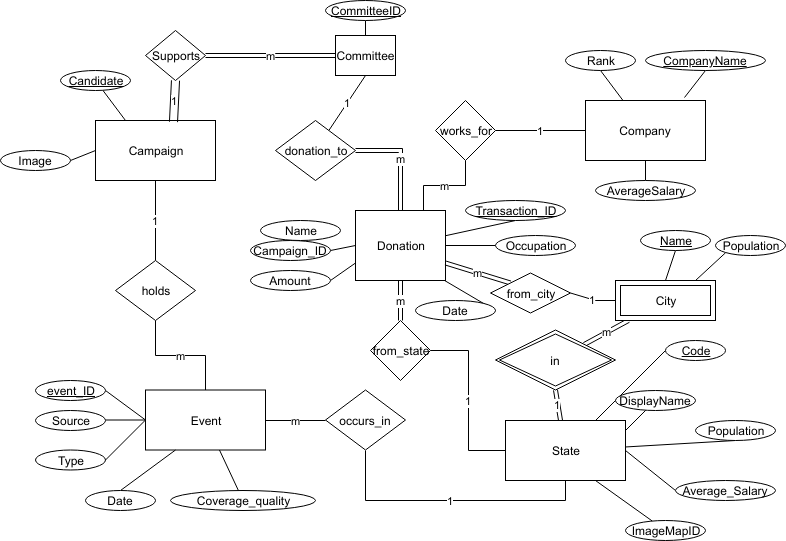
\includegraphics[scale=.40]{projecter}
        \caption{Project ER Model}
        \label{fig:projecter}
        \end{center}
    \end{figure}
\section{Schema}
\begin{verbatim}
Donation(TransactionID : int, Name : varchar(38), Amount : Decimal(9,2), 
    Occupation : varchar(38), CompanyName: varchar (38), State : varchar(2),
    City : varchar(38,), CommitteeID : varchar(10), Date : date)
Company(CompanyName : varchar(38), AverageSalary(10,2), Rank : int) 
Campaign(Candidate: varchar(38), Image : blob)
Committee(CommitteeID : varchar(10), Candidate : varchar(38))
Event(EventID : int, source : varchar(100), Type : varchar(20), Date : date, 
    Quality : int)
State(Code : varchar(2), DisplayName : varchar(15), Population : int, 
    AverageSalary, decimal(10,2) ImageMapID : int)
City(Name : varchar(38), State: varchar(2), Population : int)
\end{verbatim}
\section{SQL Commands}
\begin{verbatim}
create table Donation
    (TransactionID int,
    Name varchar(38) not null,
    Amount decimal(9,2) not null,
    Occupation varchar(38),
    CompanyName varchar(38),
    State varchar(2) check (upper(State) = State),
    City varchar(38),
    CommitteeID varchar(10) not null,
    Day date not null,
    primary key (TransactionID),
    foreign key (CompanyName) references
        Company(CompanyName),
    foreign key (State) 
        references State (Code),
    foreign key (City, State)
        references City (City, State),
    foreign key (CommitteeID) 
        references Committee(CommitteeID));
\end{verbatim}
    \begin{figure}[H]
        \begin{center}
        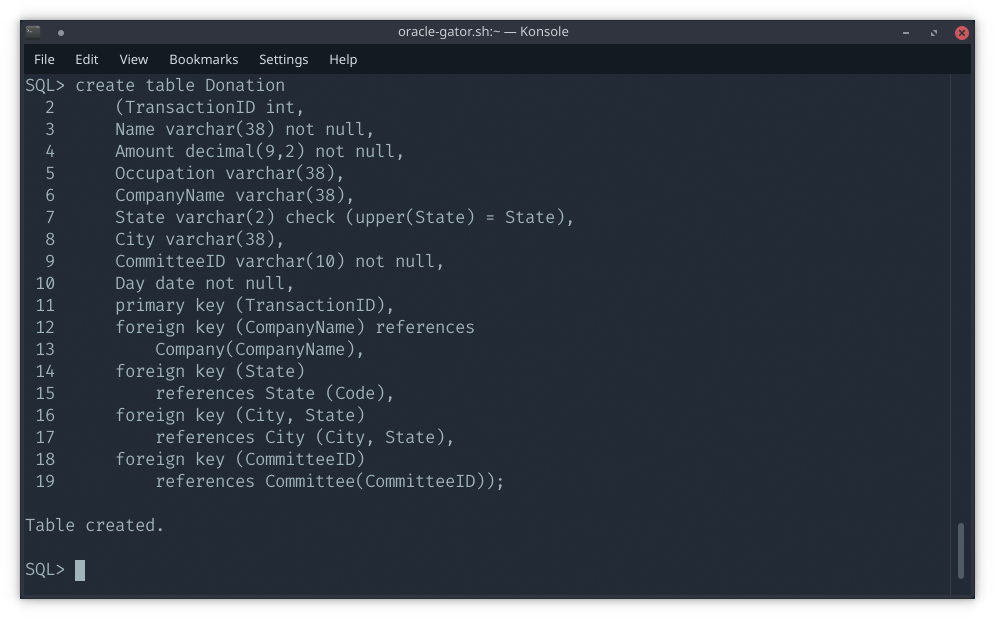
\includegraphics[scale=.40]{donation}
        \caption{Screenshot of Donation table.}
        \label{fig:donation}
        \end{center}
    \end{figure}
\begin{verbatim}
create table Company
    (CompanyName varchar(38),
    AverageSalary decimal(10,2),
    Rank int,
    primary key (CompanyName));
\end{verbatim}
    \begin{figure}[H]
        \begin{center}
        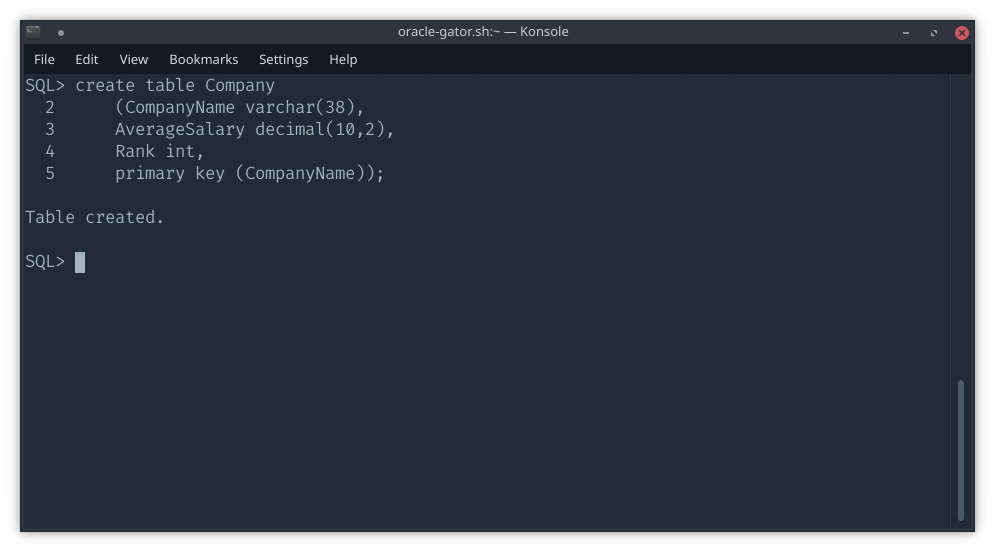
\includegraphics[scale=.40]{company}
        \caption{Screenshot of Company table.}
        \label{fig:company}
        \end{center}
    \end{figure}
\begin{verbatim}
create table Campaign
    (Candidate varchar(38),
    Image blob,
    primary key (Candidate));
\end{verbatim}
    \begin{figure}[H]
        \begin{center}
        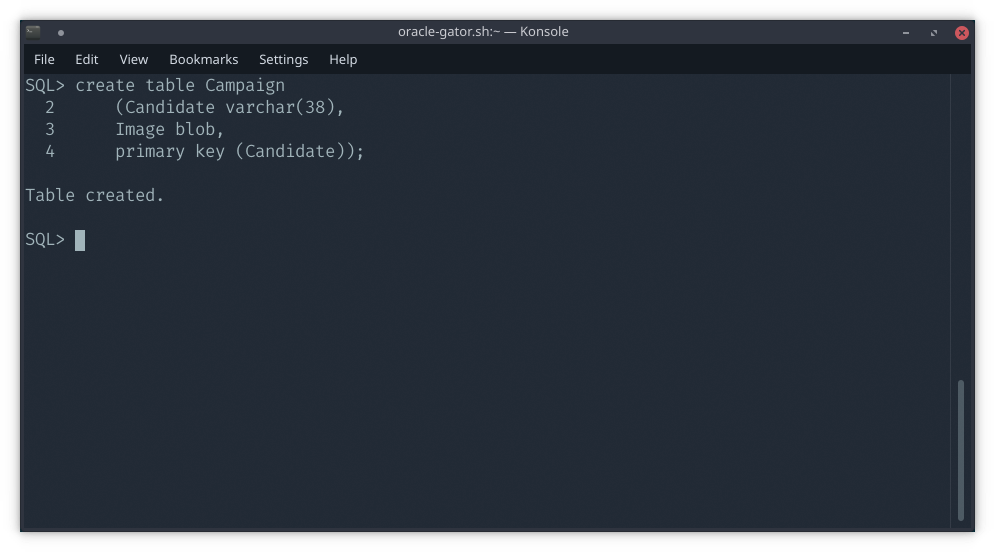
\includegraphics[scale=.40]{campaign}
        \caption{Screenshot of Campaign}
        \label{fig:campaign}
        \end{center}
    \end{figure}
\begin{verbatim}
create table Committee
    (CommitteeID varchar(10),
    Candidate varchar(38),
    primary key (CommitteeID),
    foreign key (Candidate) 
        references Campaign(Candidate));
\end{verbatim}
    \begin{figure}[H]
        \begin{center}
        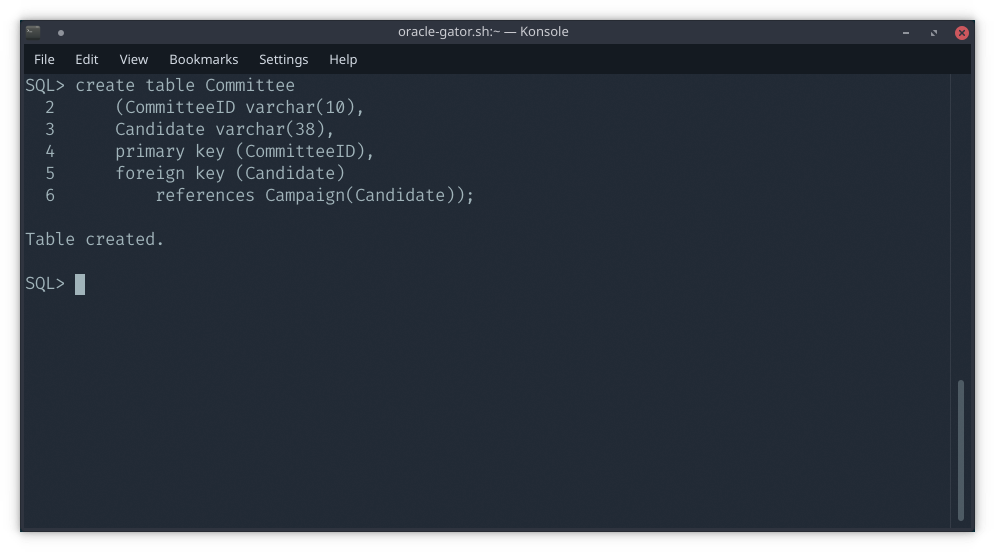
\includegraphics[scale=.40]{committee}
        \caption{Screenshot of Committee table.}
        \label{fig:committee}
        \end{center}
    \end{figure}
\pagebreak[4]
\begin{verbatim}
create table Event
    (EventID int,
    Candidate varchar(38),
    Source varchar(100),
    Type varchar(20),
    Day date,
    Quality int,
    State varchar(2);
    primary key (EventID))
    foreign key (Candidate)
        references Campaign (Candidate)
    foreign key (State)
        references State (Code));
\end{verbatim}
    \begin{figure}[H]
        \begin{center}
        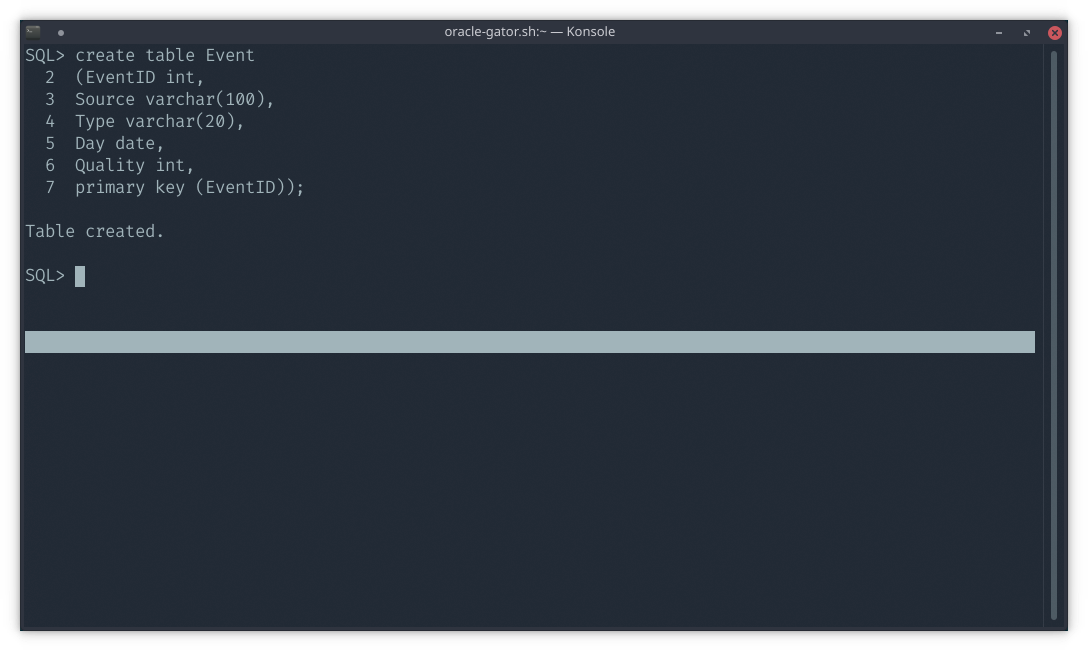
\includegraphics[scale=.40]{event}
        \caption{Screenshot of Event table.}
        \label{fig:event}
        \end{center}
    \end{figure}
\begin{verbatim}
create table State
    (Code varchar(2),
    DisplayName varchar(15),
    Population int,
    AverageSalary decimal(10,2),
    ImageMapID int,
    primary key(Code));
\end{verbatim}
    \begin{figure}[H]
        \begin{center}
        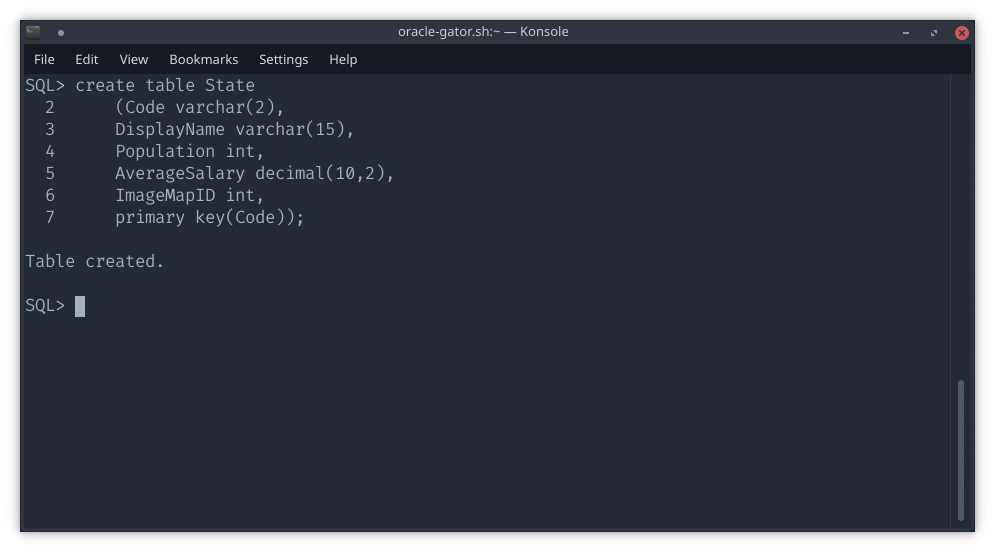
\includegraphics[scale=.40]{state}
        \caption{Screenshot of State table.}
        \label{fig:state}
        \end{center}
    \end{figure}
\begin{verbatim}
create table City
    (City varchar(38),
    State varchar(2),
    Population int,
    primary key (City, State),
    foreign key (State) 
        references State(Code));
\end{verbatim}
    \begin{figure}[H]
        \begin{center}
        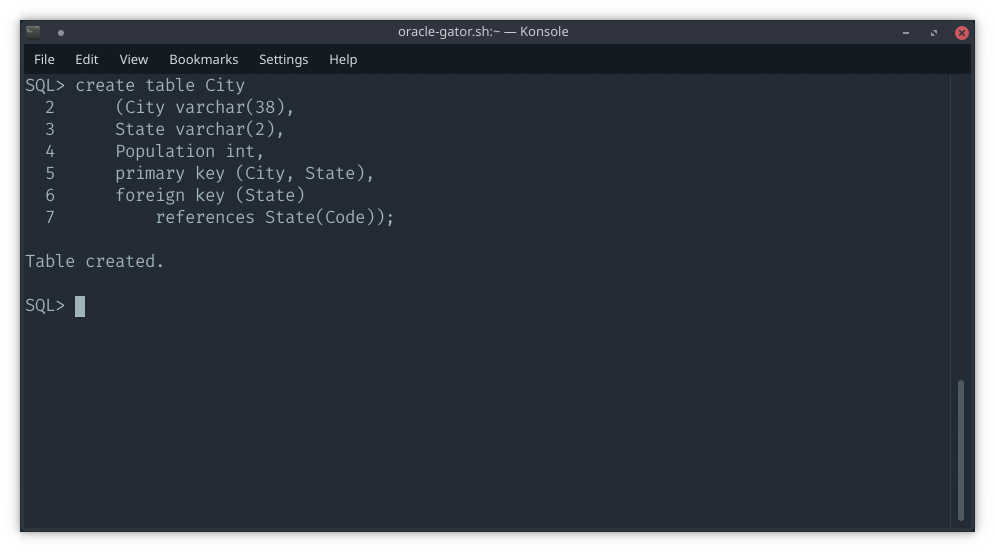
\includegraphics[scale=.40]{city}
        \caption{Screenshot of City table.}
        \label{fig:city}
        \end{center}
    \end{figure}
    \begin{verbatim}
SELECT table_name from all_tables where REGEXP_LIKE(table_name,
    'Donation|Company|Campaign|Committee|Event|State|City', 'i');
    \end{verbatim}
        \begin{figure}[H]
        \begin{center}
        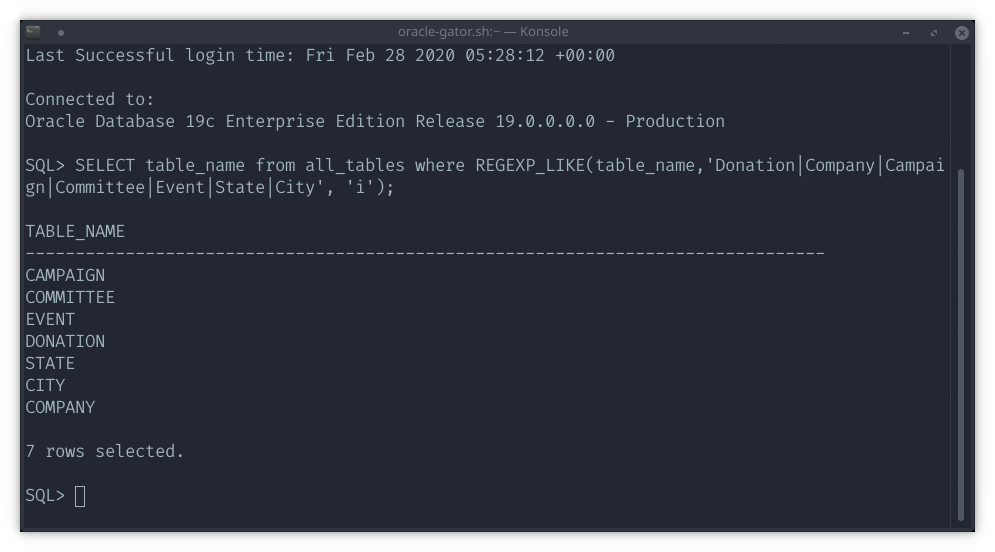
\includegraphics[scale=.40]{tables}
        \caption{Screenshot of project related tables.}
        \label{fig:tables}
        \end{center}
    \end{figure}
\end{document}
